\chapter{Implementation} 

	\section{Technologies}
		\subsection{Kivy}
			\par \textbf{Kivy}\cite{Kivy} is a \textbf{cross-platform framework} that allowed me to build the game as an \textbf{Android application}. The \textbf{relationship} between \textbf{Kivy} and \textbf{Python} reminds me heavily of the one between \textbf{CSS/HTML} and \textbf{PHP}. Placing \textbf{Widgets} in \underline{".kv"} files feels like building a \textbf{web site}. My \textbf{text-based, screen-heavy} game took \textbf{thousands} of lines of \textbf{Kivy} code. 

		\subsection{Pickle}
			\par \textbf{Pickle}\cite{Pickle} is a \textbf{Python} module used for \textbf{serializing object structures}. I used it to implement \textbf{saving, loading} and \textbf{pausing} on a \textbf{Game State object} that holds all the \textbf{information} about the \textbf{gameplay}. 
		
	\subsection{Buildozer}
		\par \textbf{Buildozer}\cite{Buildozer} is a tool that packages \textbf{mobile} applications. I used it to create the \textbf{Android executable} for the game. It requires \textbf{Linux} for compilation, so I shared the code between \textbf{Ubuntu} and \textbf{Windows} via \textbf{Github} in order to use it.
	
	\section{Integration}
		\begin{figure}[H]
			\centering
			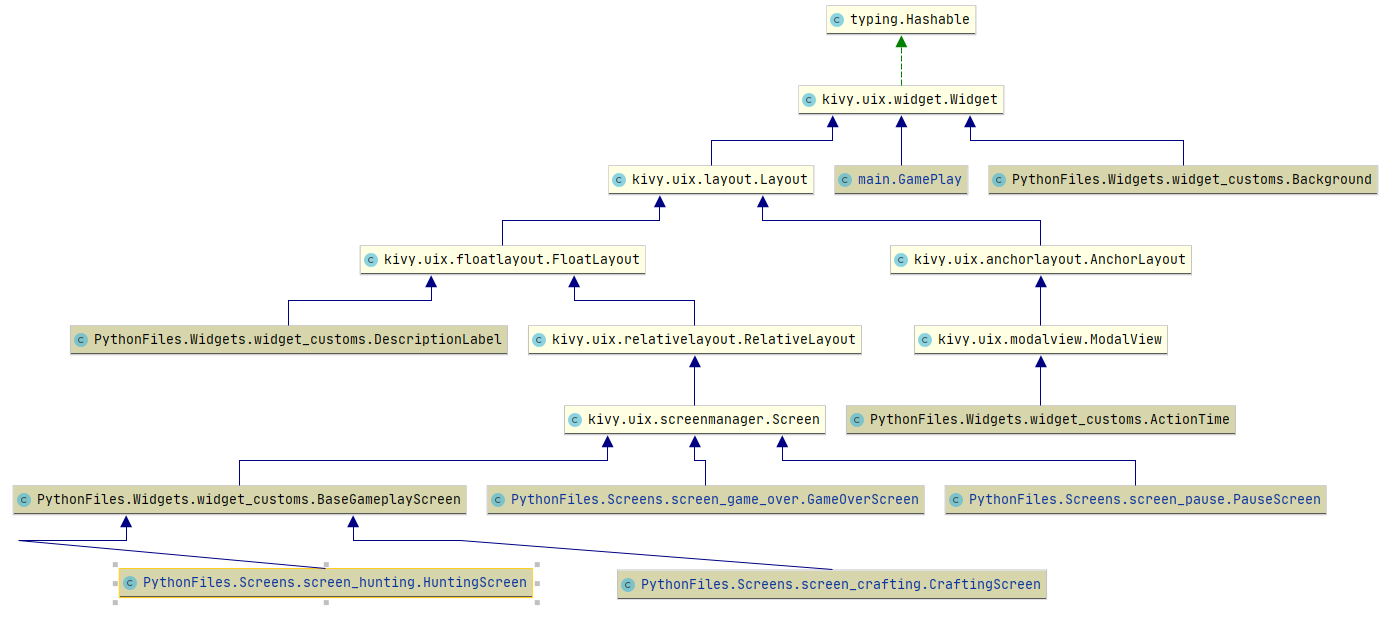
\includegraphics[width=14cm, height=9cm, keepaspectratio]{Images/Diagram.png}\\
			\caption{\textbf{Piece of Kivy and Python Integration Architecture}}
		\end{figure}
		\par \textbf{Python} makes use of \textbf{Kivy Widgets} in order to create \textbf{UI elements}. This can be seen in \textit{Figure 3.1}, which contains a piece of \textbf{integration architecture}(with most elements discarded to fit).
	
		\subsection{Kivy Using Kivy Files}
			\par \textbf{Kivy} code can be written in both \underline{".kv"} and \underline{".py"} files. \textit{Listing 3.1} displays a piece of code that adds a \textbf{Button Widget} and an \textbf{Image Widget}(a "pause" symbol) to three selected \textbf{screens}.
			\par The language's \textbf{structure} resembles \textbf{HTML}. It allows for compact code as \textbf{multiple screens} can share the same \textbf{Widgets}. The \underline{"root.show\_info()"} line calls the \underline{"show\_info()"} \textbf{method} of the \textbf{parent object} found in a ".py" file. The \underline{"on\_release"} line allows behaviour addition and makes the button \textbf{responsive}. The \textbf{image} is added on top and does not \textbf{interfere} with the \textbf{functionality} of the \textbf{button}.
			\begin{lstlisting}[caption={\textbf{Kivy} Implementation of the \textbf{Pause Button}},captionpos=b]
<FireScreen, HuntingScreen, ShelterScreen>:
    FloatLayout:
        Button:
            pos_hint:{"x": 0.91, "y": 0.90}
            size_hint: 0.04, 0.07
            background_color: 0.0, 0.0, 0.0, 1.0
            bold: True
            font_size: self.height*0.5
            text: ""
            on_release:
                root.show_info()
        Image:
            source: "GraphicFiles/info.png"
            size_hint: 0.026, 0.054
            pos_hint:{"x": 0.917, "y": 0.908}
            allow_stretch: True
			\end{lstlisting}

		\subsection{Kivy Using Python Files}
		\par \textbf{Widgets} can be \textbf{implemented} in \underline{".py"} files as well. \textbf{"ModalView"} creates a \textbf{Pop Up} the size of the current window. The code in \textit{Listing 3.2} implements a \textbf{"ModalView"} that displays an \textbf{"action execution"} text and \textbf{closes} after a second("Building...", "Sleeping...").
			\begin{lstlisting}[caption={\textbf{Kivy} Implementation of the\textbf{Action Execution Pop Up}},captionpos=b]
class ActionTime(ModalView):

    def __init__(self, text, **kwargs):
        super(ActionTime, self).__init__(**kwargs)

        # Set the specific text for the action
        self.ids.action_time_label.text = text

        # Call dismiss_view after one second
        Clock.schedule_once(self.dismiss_view, 1)

    def dismiss_view(self, dt):
        self.dismiss()
			\end{lstlisting}
	
			\par \textit{Listing 3.3} \textbf{showcases} the piece of code that \textbf{changes} the \textbf{background} picture to reflect the \textbf{time} of the day.
			
\begin{lstlisting}[caption={\textbf{Kivy} Implementation of the \textbf{Background Change}},captionpos=b]
class Background(Widget):
    """ Class for changing the background during the day """

    # The path to background image
    this_source = StringProperty("GraphicFiles/night.png")

    def change_background(self, *args):
        """ Change background after the day period """
        # Total game hours that have passed
        game_hours = init.game_state.game_time / 60
        # The current day of the game
        init.game_state.current_game_day = int(game_hours / 24 + 1)
        # Game hours that have passed in the current day
        game_hours_today = game_hours % 24

        # Change background image path based on the time of the day
        if game_hours_today < 2:
            self.this_source = "GraphicFiles/dawn.png"
        if game_hours_today < 7:
            self.this_source = "GraphicFiles/orange.png"
        elif game_hours_today < 10:
            self.this_source = "GraphicFiles/purple.png"
        elif game_hours_today < 12:
            self.this_source = "GraphicFiles/sunset.png"
        else:
            self.this_source = "GraphicFiles/night.png"
			\end{lstlisting}

	\section{Testing} 
		\par The \textbf{project} was \textbf{manually} tested after each \textbf{iteration}. The nature of the game allows for extremely \textbf{fast playthroughs}, as each action takes \textbf{one second} in real time. This was a \textbf{best case} scenario, as each feature could be \textbf{tested} in a matter of at most \textbf{several minutes}. Testing \textbf{automation} was not really needed.
		
		\subsection{Quality Assurance}
			\par As far as I am concerned, there are \textbf{no bugs} remaining. The addition of the \textbf{rain} \underline{".gif"} \textbf{animation} makes the \textbf{game} take a minute to \textbf{open} on \textbf{mobile devices} after the first installation, but the application is very \textbf{responsive} otherwise. \textbf{"Speedruns"} can cause \textbf{occasional} lags of 2-3 seconds, but \textbf{fast gameplay} poses no problems.

		\subsection{Playtesting}
			\par The \textbf{application} was \textbf{tested} by friends, family and other students. As I was implementing an already \textbf{successful game}, I didn't really have many \textbf{difficulties} with the \textbf{mechanics} and \textbf{gameplay design} choices. However, there are things that I \textbf{changed} to \textbf{my liking} and I made sure to \textbf{cater} to all the \textbf{complaints} and \textbf{suggestions}.
	
\newpage